\chapter{Metaheurísticas}

\framebox[\textwidth]{
	\hspace{1em}
	\vbox{
		\textbf{Leitura obrigatória:}
		\begin{itemize}
			\item \cite{ZapfelEtAl2010} -- Cap. 3 (Search heuristics).
			\item \cite{ZapfelEtAl2010} -- Cap. 4 (Metaheuristics in general).
		\end{itemize}
		
		\textbf{Leitura complementar:}
		\begin{itemize}
			\item \cite{RusselAndNorvig2010} -- Cap. 4 (Além da busca clássica).
		\end{itemize}
	}
}

\section{Introdução}

O Capítulo~\ref{cap:buscas} apresentou uma série de abordagens para a busca em espaço de estados. Estas abordagens partem de um estado inicial e exploram caminhos para encontrar um estado objetivo. Uma vez encontrado, a solução consiste na sequência de passos (ações) para se chegar no objetivo. No entanto, alguns problemas não se preocupam com o caminho até a solução. Por exemplo, no problema das 8 rainhas o que importa é a disposição final das rainhas no tabuleiro, e não a sequência de movimentos que levou a esta disposição. De fato, muitos problemas do mundo real consistem em apenas encontrar uma (ou a melhor) solução.

Quando a preocupação é apenas encontrar o estado objetivo do problema, podemos fazer uso de uma nova classe de algoritmos: as metaheurísticas. Uma metaheurística é um método heurístico de solução de problemas que pode ser aplicado a qualquer problema. Elas são comumente aplicadas a problemas de \textbf{otimização}, nos quais o objetivo é encontrar o melhor estado de acordo com uma função objetivo. Neste capítulo, trataremos qualquer estado como uma possível solução do problema, mesmo ele sendo de baixa qualidade ou violando restrições do problema. Logo, para aplicação de metaheurísticas, os termos \textit{estado} e \textit{solução} são sinônimos.

A \textbf{função objetivo} mede a qualidade de uma solução. Por exemplo, no problema das 8 rainhas a função objetivo pode ser definida como o número de rainhas que estão sendo atacadas por diferentes lados. Neste caso, queremos o menor valor possível (zero) para a função objetivo e classificamos o problema de otimização como um problema de minimização. Se definirmos a função objetivo como o número de rainhas que não conseguem atacar nenhuma outra peça, então queremos o maior valor possível (oito) e temos um problema de maximização. Em resumo, uma metaheurística explora o espaço de busca visando encontrar soluções que otimizem (minimizem ou maximizem) uma dada função objetivo.

Em geral, as metaheurísticas são aplicadas a espaços de busca grandes e até mesmo infinitos, para os quais não existem algoritmos sistemáticos adequados. Além dessa capacidade de exploração, elas consomem pouca memória, pois armazenam apenas uma ou um conjunto fixo de soluções. No entanto, as metaheurísticas não garantem completude e otimalidade. A ideia é encontrar uma solução de qualidade satisfatória, utilizando baixos recursos de tempo e armazenamento. Por conta disso, as metaheurísticas são geralmente escolhidas no tratamento de problemas NP-Completos.

As metaheurísticas podem ser classificadas de acordo com a natureza da busca que realizam:
\begin{itemize}
	\item \textbf{Busca por construção de soluções:} repetidamente constrói soluções e armazena a melhor solução construída. Uma construção pode utilizar conhecimento adquirido de iterações anteriores.
	\begin{itemize}
		\item \textbf{Exemplo das 8 rainhas:} inicia com o tabuleiro vazio e vai inserindo as peças até obter uma solução completa.
	\end{itemize}
	
	\item \textbf{Busca por modificação de soluções:} inicia com uma solução inicial e aplica modificações, de forma a melhorar a solução.
	\begin{itemize}
		\item \textbf{Exemplo das 8 rainhas:} inicia com uma disposição aleatória das peças no tabuleiro e iterativamente troca uma peça para uma posição que melhore a solução.
	\end{itemize}
	
	\item \textbf{Busca por recombinação de soluções:} mantém um conjunto de soluções na memória e aplica recombinação entre pares de soluções. Uma recombinação cria uma solução filha que herda parte da solução de cada solução recombinada. Após a fase de recombinação, seleciona a melhor população para a próxima iteração.
	\begin{itemize}
		\item \textbf{Exemplo das 8 rainhas:} mantém um conjunto de 10 soluções (diferentes disposições das peças no tabuleiro). A cada iteração, recombina cada par de soluções, tal que a solução filha posicione as quatro primeiras rainhas conforme a disposição da primeira solução geradora, e as quatro demais rainhas conforme a disposição da segunda solução geradora. Após isso, seleciona as 10 melhores soluções para a próxima iteração.
	\end{itemize}
\end{itemize}

Este capítulo foca no estudo de metaheurísticas por modificação e recombinação de soluções. Especificamente, são apresentados diferentes algoritmos de \textbf{busca local} como métodos de busca por modificação de soluções, e \textbf{algoritmos genéticos} como métodos de busca por recombinação de soluções.

\section{Busca local}

Os algoritmos de busca local recebem uma solução inicial e aplicam modificações em busca de melhorias na solução. Cada modificação é chamada de \textbf{movimento} e a solução resultante do movimento é chamada de \textbf{solução vizinha} ou simplesmente \textbf{vizinho}. O Algoritmo~\ref{alg:busca-local} apresenta o pseudocódigo para uma busca local considerando como objetivo a minimização da função objetivo $\varphi(s)$.

\begin{algorithm}[h]
	\DontPrintSemicolon
	\Entrada{\textit{solução inicial} -- $s$}
	\Saida{\textit{melhor solução encontrada} -- $s^*$}
	
	\Inicio{
		$s^* \gets s$\;
		\Enqto{critério de parada não satisfeito}{
			seleciona vizinho $s' \in N(s)$ de acordo com \textbf{estratégia de seleção}\;
			$s \gets s'$\;
			\Se{$\varphi(s) < \varphi(s^*)$}{
				$s* \gets s$\;
			}
		}
		\Retorna{$s^*$}
	}
	
	\caption{Pseudocódigo para uma busca local}
	\label{alg:busca-local}
\end{algorithm}

A \textit{solução inicial} $s$ consiste em uma solução com um estado válido do espaço de busca. O algoritmo mantém a melhor solução conhecida em $s^*$, que é retornada no final da execução. Enquanto um determinado critério de parada não é satisfeito, o algoritmo seleciona um vizinho $s'$ (linha 4) e, caso ele seja melhor que a melhor solução conhecida, ela é substituída (linhas 5, 6 e 7).

Para termos uma instância de uma busca local, temos que determinar a \textbf{forma como os vizinhos são gerados} e a \textbf{estratégia de seleção} do vizinho a cada iteração. Em geral, o projetista define um ou um conjunto de operadores que, aplicados à solução, geram um vizinho. Por exemplo, dada uma solução para o problema das 8 rainhas, um operador válido consiste em selecionar uma rainha e movê-la para uma casa adjacente. A aplicação deste operador gera um grande número de vizinhos diferentes, pois podemos selecionar cada vez uma das rainhas e cada vez uma das casas adjacentes. O conjunto de todos os vizinhos gerados pelo(s) operador(es) utilizado(s) é chamado de \textbf{vizinhança} da solução e está representada por $N(s)$ no Algoritmo~\ref{alg:busca-local}.

Uma vez definida a vizinhança utilizada $N(s)$ (o conjunto de operadores adotados), temos que definir a estratégia de seleção de um vizinho $s' \in N(s)$. Uma busca local simples sempre seleciona um vizinho que melhora o valor da função objetivo. Por conta disso, esta busca local é conhecida como \textbf{subida da montanha}\footnote{O algoritmo de subida da montanha geralmente propõe o uso da estratégia de seleção \textbf{melhora aleatória}.} (ou \textbf{hill climbing}), pois faz uma analogia de que a busca tenta sempre melhorar a qualidade da solução e, portanto, sempre sobe. Outros nomes decorrentes desta característica são \textbf{busca local gulosa} e \textbf{busca local monótona}. Apesar de sua simplicidade, existem diferentes estratégias para selecionar um vizinho melhor, as principais são apresentadas na sequência.

\begin{itemize}
	\item \textbf{Primeira melhora:} seleciona o primeiro vizinho que proporciona alguma melhora, isto é, que satisfaz $\varphi(s') < \varphi(s)$ para um problema de minimização. Esta estratégia não necessita que todos os vizinhos sejam gerados.
	
	\item \textbf{Melhor melhora:} seleciona o melhor vizinho de toda a vizinhança, isto é, aquele que apresenta o menor valor de $\varphi(s)$ para um problema de minimização. Esta estratégia exige que toda a vizinhança seja gerada.
	
	\item \textbf{Melhora aleatória:} seleciona aleatoriamente um dos vizinhos que proporciona alguma melhora. Esta abordagem também não exige a geração de toda a vizinhança.
\end{itemize}


\subsection{Topologia da vizinhança}

Para entender o funcionamento e o desempenho de buscas locais, é necessário considerar a topologia do espaço de busca (ou espaço de estados), que é definida em função da vizinhança adotada. A Figura~\ref{fig:topologia-espaco-busca} apresenta uma representação de um espaço de busca unidimensional, onde o eixo $x$ define o espaço de estados e o eixo $y$ mapeia o valor da função objetivo. Dois estados vizinhos no eixo $x$ são também vizinhos na busca local.

\begin{figure}[h]
	\centering
	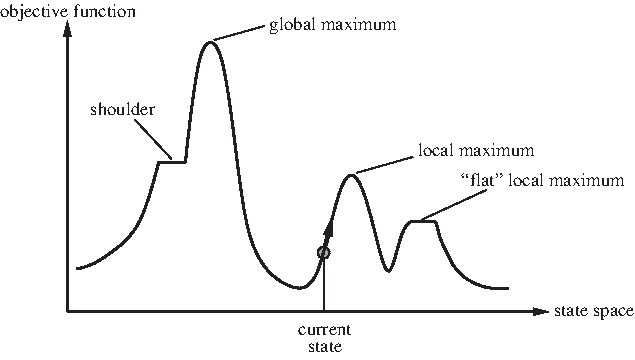
\includegraphics[width=0.75\textwidth]{img/topologia-espaco-busca}
	\caption{Uma representação da topologia de um espaço de estados unidimensional}
	\label{fig:topologia-espaco-busca}
\end{figure}

Considerando este espaço de busca para um problema de maximização, queremos encontrar a solução com maior valor possível para a função objetivo. Esta solução é chamada de máximo global e está representada na Figura~\ref{fig:topologia-espaco-busca}. O máximo global, além de ser o estado (ou a solução) que possui maior valor para a função objetivo, tem a característica de que todos os seus vizinhos possuem valor de função objetivo menores ou iguais ao seu. Portanto, se a busca encontrar uma solução com esta segunda característica, sabemos que trata-se de um máximo, mas não podemos garantir que este seja o máximo global, pois pode ocorrer em outras regiões do espaço de busca e não possuir o maior valor para a função objetivo. Neste caso, trata-se de um máximo local, também representado na Figura~\ref{fig:topologia-espaco-busca}. Finalmente, existem regiões em que as todas as soluções vizinhas possuem o mesmo valor de função objetivo. Este caso é chamado de platô (ou \textit{plateau}), ou ainda planície (representado pela região \textit{shoulder} na Figura~\ref{fig:topologia-espaco-busca}).

Conhecer as possíveis situações que a busca vai encontrar em diferentes topologias é importante para entender as limitações de uma busca local e os casos específicos com os quais se preocupar. Como a busca local somente seleciona vizinhos que melhoram a função objetivo, caso ela encontre um máximo local, não conseguirá ``sair'' desta solução. Observe o estado atual representado na Figura~\ref{fig:topologia-espaco-busca}. Esta solução encontra-se subindo na sua vizinhança, pois a busca tenta sempre melhorá-la. Ao chegar no máximo local, nenhum vizinho possui um melhor (maior) valor de função objetivo e a busca termina. No entanto, esta não é a melhor solução para o problema. A mesma situação acontece em platôs, onde uma busca local simples não é capaz de superá-los.

Portanto, uma busca local simples, do tipo subida da encosta, tem como critério de parada o fato de encontrar uma solução ótima, que não é garantidamente o ótimo global do problema. Esta é a deficiência desta busca e diferentes estratégias são adotadas para superá-la, dando origem às variantes da busca local.

\subsection{Exemplo: problema das 8 rainhas}

Consideremos o problema das 8-rainhas. É sabido que duas rainhas não podem estar na mesma linha ou coluna. Portanto, uma boa estratégia consiste em distribuir inicialmente cada rainha em uma das colunas e em linhas aleatórias gerando, assim, a solução inicial. Cada rainha permanece na sua coluna, portanto o movimento consiste em selecionar uma rainha e movê-la para outro quadrado da mesma coluna. Cada estado possui $8 \times 7 = 56$ estados sucessores, que compõem sua vizinhança. A função objetivo pode ser definida como o número de pares de rainhas que estão se atacando. O mínimo global dessa função é zero, que só ocorre em soluções perfeitas.

A Figura~\ref{fig:busca-local-oito-rainhas} mostra um possível estado para o problema, cuja função objetivo possui valor $17$. No tabuleiro, são apresentados os valores da função objetivo das soluções vizinhas. Percebe-se que alguns movimentos diminuem a função objetivo para $12$, que é a melhor melhora possível. Uma busca local, portanto, seleciona vizinhos que melhoram o valor da função objetivo de acordo com alguma das estratégias apresentadas.

\begin{figure}[h]
	\centering
	\hspace{15pt}
	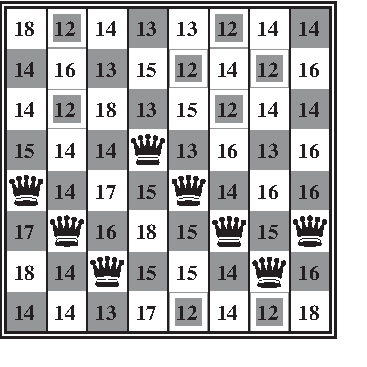
\includegraphics[width=0.5\textwidth]{img/busca-local-oito-rainhas}
	\caption{Uma solução parcial com custos para o problema das 8 rainhas}
	\label{fig:busca-local-oito-rainhas}
\end{figure}

Conforme discutido nas seções anteriores, a deficiência da busca local simples (subida da montanha) é a incapacidade de superar ótimos locais. O espaço de busca do problema das 8 rainhas é caracterizado por muitos mínimos locais, o que dificulta o desempenho da busca local. A Figura~\ref{fig:minimo-local-oito-rainhas} apresenta um mínimo local para o problema das 8 rainhas, cuja função objetivo soma $1$ (muito próximo da solução), mas todos os vizinhos possuem valores maiores.

\begin{figure}[h]
	\centering
	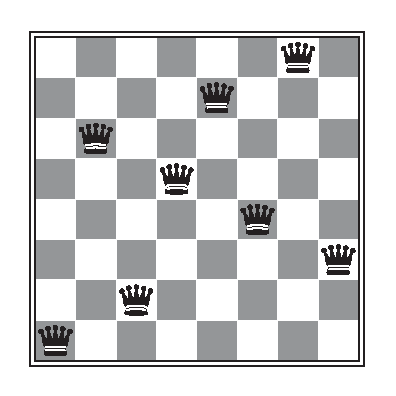
\includegraphics[width=0.55\textwidth]{img/minimo-local-oito-rainhas}
	\caption{Um mínimo local para o problema das 8 rainhas}
	\label{fig:minimo-local-oito-rainhas}
\end{figure}

Devido à topologia do seu espaço de estados, uma busca local retorna um ótimo local em aproximadamente 86\% dos casos para o problema das 8 rainhas e, portanto, resolve em apenas 14\% das vezes. Apesar disso, a convergência é rápida, pois a busca demora cerca de quatro passos quando encontra a solução ótima, e três passos quando encontra um ótimo local. Isso mostra o potencial da busca local, pois o espaço de busca contém $8^8 \approx 17$ milhões de estados.

Para chegar à solução ótima, o algoritmo deve adotar alguma estratégia para superar ótimos locais. Por exemplo, a busca poderia permitir soluções piores, visando uma melhora futura. As próximas seções apresentam variantes da busca local com o objetivo de superar esta deficiência.

\subsection{Busca local randomizada}

Uma primeira estratégia para superar ótimos locais consiste em incluir um componente aleatório que permite selecionar vizinhos iguais ou piores. Neste sentido, a busca local randomizada (ou \textbf{busca local estocástica}) recebe um parâmetro $p \in [0,1]$ como entrada, que define a probabilidade da busca fazer um movimento aleatório. Com probabilidade $p$ a busca seleciona um vizinho qualquer, e com probabilidade $1 - p$ a busca escolhe um vizinho melhor de acordo com alguma sub-estratégia de seleção (primeira melhora, melhor melhora ou melhora aleatória).

\begin{algorithm}[h]
	\DontPrintSemicolon
	\Entrada{\textit{solução inicial} -- $s$, \textit{probabilidade} -- $p$}
	\Saida{\textit{melhor solução encontrada} -- $s^*$}
	
	\Inicio{
		$s^* \gets s$\;
		\Enqto{critério de parada não satisfeito}{
			num $\gets$ randomFloat() \textit{//de 0 a 1}\;
			\Se{num $\le p$}{
				seleciona qualquer vizinho $s' \in N(s)$\;
			}
			\Senao{
				seleciona vizinho melhor $s' \in N(s)$\;
			}
			
			$s \gets s'$\;
			\Se{$\varphi(s) < \varphi(s^*)$}{
				$s* \gets s$\;
			}
		}
		\Retorna{$s^*$}
	}
	
	\caption{Pseudocódigo para uma busca local randomizada}
	\label{alg:busca-local-randomizada}
\end{algorithm}

O Algoritmo~\ref{alg:busca-local-randomizada} apresenta o pseudocódigo para uma busca local randomizada. A estratégia de randomização é implementada nas linhas 4 a 8, que seleciona os vizinhos em função da probabilidade $p$. Apesar de simples, esta estratégia consegue superar ótimos locais. No entanto, exigindo a calibração de $p$\footnote{Perceba que assumindo $p = 0$, temos uma busca local simples, enquanto com $p = 1$ temos uma \textbf{caminhada aleatória} no espaço de busca.}. O critério de parada pode ser a qualidade da melhor solução conhecida, o número de iterações sem melhora, o número máximo de iterações ou um limite em tempo de execução.

\subsection{Busca local iterada}

Uma segunda abordagem consiste em reiniciar a busca sempre que ela encontra um ótimo local. Isto é, executar a busca local repetidamente de forma a, em uma das execuções, encontrar o ótimo global. Uma alternativa mais interessante consiste em executar uma busca local iterativamente, alterando parte da solução sempre que um ótimo local for encontrado. Esta alteração é chamada de \textbf{perturbação} e o algoritmo é chamado de busca local iterada (\textbf{iterated local search}). Seu funcionamento é expresso no Algoritmo~\ref{alg:busca-local-iterada}.

\begin{algorithm}[h]
	\DontPrintSemicolon
	\Entrada{\textit{solução inicial} -- $s$}
	\Saida{\textit{melhor solução encontrada} -- $s^*$}
	
	\Inicio{
		$s^* \gets s$\;
		\Enqto{critério de parada não satisfeito}{
			s $\gets$ perturba($s$)\;
			s $\gets$ buscaLocal($s$)\;
			\Se{$\varphi(s) < \varphi(s^*)$}{
				$s* \gets s$\;
			}
		}
		\Retorna{$s^*$}
	}
	
	\caption{Pseudocódigo para uma busca local iterada}
	\label{alg:busca-local-iterada}
\end{algorithm}

Em resumo, uma busca local iterada repetidamente perturba uma solução e aplica uma busca local, armazenando a melhor solução encontrada. A perturbação consiste em modificar a solução de forma que na próxima busca local, outro ótimo seja encontrado. Um parâmetro que pode ser incluído na busca é o tamanho da perturbação, isto é, quanto da solução será modificada. No problema das 8 rainhas, por exemplo, uma possível perturbação consiste em selecionar parte das rainhas e mover para uma posição aleatória da mesma coluna. O critério de parada pode ser a qualidade da melhor solução conhecida, o número de iterações sem melhora, o número máximo de iterações ou um limite em tempo de execução.

\subsection{Simulated annealing}

As estratégias de busca local randomizada e busca local iterada tornam a busca completa, mas podem se apresentar ineficientes de acordo com o tamanho e topologia do espaço de busca. O algoritmo de simulated annealing (ou \textbf{têmpera simulada}) é uma tentativa de obter completude de forma mais eficiente. Esta abordagem foi proposta por \citet{KirkpatrickEtAl1983} e \citet{Cerny1985} e faz uma analogia à evolução de um sólido para o equilíbrio térmico, no processo conhecido como têmpera ou arrefecimento de metais. A ideia básica consiste em explorar o espaço de busca, aceitando soluções piores com maior probabilidade no início e decrescendo esta probabilidade com o passar do tempo, similar à diminuição de temperatura de uma têmpera.

O simulated annealing utiliza o \textbf{critério de aceitação de Metropolis}~\citep{MetropolisEtAl1953}, dado por:
$$
P[\text{aceitar } s' \mid s] = 
\begin{cases}
	1  & \text{caso } s' \text{ seja melhor que } s \\
	e^{-\Delta(s, s')/T}  & \text{caso contrário.}
\end{cases}
$$
Caso a nova solução $s'$ seja melhor, ela é sempre aceita. Caso ela seja pior, a probabilidade de ela ser aceita varia em função do quanto ela piora a solução atual $\Delta(s, s') = \varphi(s') - \varphi(s)$ e da temperatura $T$. A temperatura evolui, diminuindo a cada iteração. Dessa forma, no início a busca aceita mais soluções piores, enquanto no final a busca é intensificada (para soluções de melhor qualidade).

\begin{algorithm}[h]
	\DontPrintSemicolon
	\Entrada{\textit{solução inicial} -- $s$, \textit{temperatura inicial} -- $T_0$, \textit{temperatura final} -- $T_{final}$}
	\Saida{\textit{melhor solução encontrada} -- $s^*$}
	
	\Inicio{
		$s^* \gets s$\;
		$T \gets T_0$
		
		\Enqto{$T > T_{final}$}{
			seleciona vizinho $s' \in N(s)$ aleatoriamente\;
			\Se{$\Delta(s, s') <= 0$}{
				$s \gets s'$\;
			}
			\Senao{
				$s \gets s'$ com probabilidade $e^{-\Delta(s, s')/T}$\;
			}
			
			\Se{$\varphi(s) < \varphi(s^*)$}{
				$s* \gets s$\;
			}
			
			$T \gets$ proximaTemperatura($T$)\;
		}
		\Retorna{$s^*$}
	}
	
	\caption{Pseudocódigo para o algoritmo de simulated annealing}
	\label{alg:simulated-annealing}
\end{algorithm}

O Algoritmo~\ref{alg:simulated-annealing} apresenta o pseudocódigo do simulated annealing. Os parâmetros $T$, $T_{final}$ e a definição da estratégia de atualização de temperatura (linha 12) devem ser ajustados empiricamente, pois sua performance varia em função do problema. \citet{RusselAndNorvig2010} explicam didaticamente o método de simulated annealing da seguinte forma:

\begin{quotation}
``\textit{Para explicar a têmpera simulada, vamos mudar nosso ponto de vista de subida de encosta para descida de gradiente (isto é, minimização do custo) e imaginar a tarefa de colocar uma bola de pingue-pongue na fenda mais profunda em uma superfície acidentada. Se simplesmente deixarmos a bola rolar, ela acabará em um mínimo local. Se agitarmos a superfície, poderemos fazer a bola quicar para fora do mínimo local. O artifício é agitar com força suficiente para fazer a bola sair dos mínimos locais, mas não o bastante para desalojá-la do mínimo global. A solução de têmpera simulada é começar a agitar com força (isto é, em alta temperatura) e depois reduzir gradualmente a intensidade da agitação (ou seja, baixar a temperatura).}''
\end{quotation}

\section{Algoritmos genéticos}

Os algoritmos genéticos fazem parte de uma área de estudos chamada \textbf{computação evolucionária} (veja mais detalhes em \citet{EibenAndSmith2003}) e são uma metaheurística baseada em recombinação de soluções. Suas ideias se baseiam na teoria da evolução de Darwin e no mecanismo de seleção natural que fazem com que as espécies evoluam. Dessa forma, os algoritmos genéticos propõem a evolução de soluções mediante o processo de seleção natural. Por conta disso, esta abordagem compõe, juntamente com outras áreas da computação e da inteligência artificial, uma vertente chamada computação bioinspirada, ou computação baseada na natureza.

Em resumo, os seres vivos competem entre si por recursos limitados. Nesta competição, apenas os indivíduos mais aptos sobrevivem (seleção natural). Os seres vivos se reproduzem, gerando descendentes que herdam as características dos pais. Logo, as características de aptidão são passadas para as próximas gerações. Esta seção apresenta a forma como estes conceitos são aplicados aos algoritmos genéticos para a solução de problemas de otimização.

\subsection{Esquema geral}

Podemos decompor um algoritmo genético nas etapas ilustradas na Figura~\ref{fig:algoritmo-genetico}. Cada etapa é apresentada como um bloco, juntamente com o fluxo de execução entre elas. A população é composta por soluções viáveis do problema, isto é, estados possíveis para o problema. Na primeira etapa esta população é inicializada, ou seja, são criadas várias soluções, conforme o tamanho desejado para a população. Para cada indivíduo, é calculada sua aptidão (segunda etapa), que consiste na qualidade da solução. Caso algum critério de terminação seja satisfeito, a busca termina. Como critérios de terminação pode-se definir um número máximo de iterações, tempo limite, qualidade mínima da melhor solução encontrada, número máximo de iterações sem aumento significativo da aptidão máxima da população, entre outras.

\begin{figure}[H]
	\centering
	
	\tikzstyle{decision} = [diamond, draw, fill=blue!20, text width=6em, text badly centered, node distance=3cm, inner sep=0pt]
	\tikzstyle{block} = [rectangle, draw, fill=blue!20, text width=6.4em, text centered, rounded corners, minimum height=4em]
	\tikzstyle{line} = [draw, -latex']
	\tikzstyle{cloud} = [draw, ellipse,fill=red!20, node distance=3cm, minimum height=2em]	
	
	\begin{tikzpicture}[node distance = 2.5cm, auto]
		\node [block] (inicializa) {Inicializa população};
		\node [block, below of=inicializa] (aptidao) {Calcula aptidão};
		\node [decision, below of=aptidao, node distance=3.5cm] (terminacao) {Critério terminação?};
		\node [block, below of=terminacao, node distance=3.5cm] (selecao) {Seleção};
		\node [block, below of=selecao] (recombinacao) {Recombinação};
		\node [block, below of=recombinacao] (mutacao) {Mutação};
		\node [block, below of=mutacao] (substitui) {Substitui população};
		\node [left of=selecao, node distance=4cm] (temp) {Nova geração};
		\node [block, right of=terminacao, node distance=4.5cm] (fim) {Fim};
		
		\path [line] (inicializa) -- (aptidao);
		\path [line] (aptidao) -- (terminacao);
		\path [line] (terminacao) -- node {não}(selecao);
		\path [line] (selecao) -- (recombinacao);
		\path [line] (recombinacao) -- (mutacao);
		\path [line] (mutacao) -- (substitui);
		\draw (substitui) -| (temp);
		\path [line] (temp) |- (aptidao);
		\path [line] (terminacao) -- node {sim}(fim);
	\end{tikzpicture}
	
	\caption{Esquema geral de um algoritmo genético}
	\label{fig:algoritmo-genetico}
\end{figure}

Enquanto a busca não termina, parte da população é selecionada para a recombinação (terceira etapa). O número de indivíduos selecionados pode ser uma quantidade fixa ou um percentual do tamanho da população. A escolha de quais indivíduos serão selecionados é realizada em função do valor de aptidão de cada um (ex: indivíduos mais aptos recombinam). Cada par\footnote{Um número diferente de indivíduos pode ser utilizado na recombinação. Ex: três indivíduos recombinam e geram dois filhos.} de indivíduos selecionados é recombinado (quarta etapa), gerando novos indivíduos.

Os indivíduos que fazem parte da população e os indivíduos gerados podem sofrer uma mutação, que consiste na alteração de parte da solução. A mutação é utilizada como fator de diversificação da busca, similar à perturbação utilizada na busca local iterada. Finalmente, são selecionados os indivíduos (da população original e dos novos) para comporem a nova população. Esta seleção é geralmente realizada em função da aptidão dos indivíduos (os mais aptos, mais um pequeno grupo de menos aptos para diversificação). Este mesmo esquema geral está expresso no Algoritmo~\ref{alg:algoritmo-genetico}.

\begin{algorithm}[h]
	\DontPrintSemicolon
	\Entrada{\textit{parâmetros das etapas}}
	\Saida{\textit{melhor solução encontrada}}
	
	\Inicio{
		populacao $\gets$ inicializaPopulacao()\;
		calculaAptidao(populacao)\;
		
		\Se{critério de terminação satisfeito}{
			\Retorna{melhor solução da população}	
		}
		
		popRecombinar $\gets$ selecao(populacao)\;
		novosIndividuos $\gets$ recombinacao(popRecombinar)\;
		mutacao(populacao $\cup$ novosIndividuos)\;
		populacao $\gets$ substitui(populacao $\cup$ novosIndividuos)\;
	}
	
	\caption{Pseudocódigo para um algoritmo genético}
	\label{alg:algoritmo-genetico}
\end{algorithm}

As próximas seções apresentam os componentes que precisam ser projetados para o desenvolvimento de um algoritmo genético, bem como detalham as etapas discutidas nesta seção.

\subsection{Representação de estados/soluções}

Para exemplificar os passos na construção de um algoritmo genético, vamos considerar um problema simples de maximizar a função $f(x) = x^2$, com o domínio de $x \in [0, 63]$. Chamaremos este problema de ``maximização de função quadrática'' e podemos formalizá-lo como
$$
\begin{aligned}
	& \text{maximiza} & & f(x) = x^2 \\
	& \text{sujeito a} & & x \in [0, 63].
\end{aligned}
$$

Uma vez definido o problema a ser tratado, o primeiro passo consiste em determinar uma \textbf{representação cromossomial} (ou representação na forma de cromossomo) para a solução (estado). Consiste em uma representação \textbf{sequencial}, que permita realizar as operações de cálculo de aptidão, cruzamento (recombinação) e mutação. Para o problema da maximização de função quadrática, temos 64 soluções diferentes, que são números inteiros de 0 a 63. Uma representação cromossomial comum é a representação binária, que pode ser utilizada para representar o domínio em questão. Sendo assim, precisamos de 6 bits para representar o intervalo desejado. Por exemplo, o número 0 é representado por \texttt{000000}, o número 11 é representado por \texttt{001011}, o número 46 é representado por \texttt{101110} e o número 63 é representado por \texttt{111111}. A solução original (representação decimal) é chamada de \textbf{fenótipo}, sua representação sequencial é chamada de \textbf{cromossomo} e cada posição desta sequência é chamado de \textbf{gene}. Logo, cada valor binário dos exemplos anteriores é um gene do cromossomo, que é composto por 6 genes.

Apesar da maioria dos algoritmos genéticos utilizar uma representação binária, isso não é uma regra. É possível definir outras formas de representação sequencial. O problema das 8 rainhas, por exemplo, pode ser representado por um vetor de inteiros de 8 posições. Cada posição $i$ armazena valores de $1$ a $8$, que representam o quadrado que a rainha $i$ ocupa na coluna $i$.

Além da representação da solução, é preciso definir a função objetivo, que calcula a qualidade da solução. No contexto dos algoritmos genéticos, a função objetivo é chamada de \textbf{função de fitness} e a qualidade da solução é chamada de \textbf{fitness} ou \textbf{aptidão}. No caso do problema de maximização de função quadrática, a função de fitness é a própria função $f(x) = x^2$. Por exemplo, a solução $0 =$ \texttt{000000} possui fitness de $0$. A solução $11 =$ \texttt{001011} possui fitness de $121$. A solução $46 =$ \texttt{101110} possui fitness de 2116. A solução $63 =$ \texttt{111111} possui fitness de 3969 e, obviamente, é a solução ótima.

\textbf{Observação:} perceba que em um problema de minimização, quanto menor o valor da função objetivo, maior a qualidade da solução. Neste caso, a função de fitness pode ser definida como a inversa da função objetivo ($1/\varphi(s)$). Caso contrário, as demais etapas devem ser ajustadas para tratar uma função de fitness de minimização.

\subsection{Seleção de indivíduos}

A etapa de seleção define quais indivíduos serão utilizados para a recombinação. A estratégia mais simples consiste em selecionar todos os indivíduos. No entanto, esta abordagem pode ser ineficiente, pois o tempo de processamento é alto. Outra abordagem consiste em selecionar apenas parte da população. Selecionar apenas os indivíduos com maior aptidão não é adequado, pois pode enviesar a busca. O ideal é selecionar os bons indivíduos e alguns com menor aptidão para diversidade.

Uma abordagem simples consiste em selecionar os 50\% melhores indivíduos, juntamente com os 10\% piores (estes percentuais podem ser ajustados). Uma segunda abordagem seleciona indivíduos probabilisticamente. Quanto maior a aptidão do indivíduo, maior a probabilidade de ser selecionado. Uma proposta amplamente utilizada é
$$
P[\text{selecionar } i] = \frac{fitness(i)}{\sum_{j} fitness(j)}
$$

\begin{table}[h]
	\centering
	
	\begin{tabular}{L{3cm}R{2.5cm}R{2.5cm}R{4.5cm}}
		\hline
		\textbf{Cromossomo} & \textbf{Fenótipo} & \textbf{Fitness} & $P[\text{selecionar }i]$ \\
		\hline
		\texttt{000000} & 0 & 0 & 0 \\
		\texttt{001011} & 11 & 121 & $121/6206 = 0,02$ \\
		\texttt{101110} & 46 & 2116 & $2116/6206 = 0,34$ \\
		\texttt{111111} & 63 & 3969 & $3969/6206 = 0,64$ \\
		\hline
	\end{tabular}
	
	\caption{Exemplo de seleção probabilística para a maximização de função quadrática}
	\label{tab:selecao-probabilistica}
\end{table}

\insertspace

A Tabela~\ref{tab:selecao-probabilistica} mostra quatro soluções para o problema de maximização de função quadrática, com o respectivo fitness e a probabilidade de seleção de recombinação. O somatório dos valores de fitness é 6206. Perceba que qualquer solução (exceto com fitness 0) pode ser selecionada. A seleção apenas prioriza soluções com maior aptidão.

Uma abordagem para a implementação de decisões probabilísticas é chamado de \textbf{método da roleta}. Consiste em definir o intervalo de valores para seleção dos indivíduos. A Tabela~\ref{tab:selecao-probabilistica-roleta} mostra a probabilidade acumulada de cada indivíduo, isto é, a sua probabilidade somada às probabilidades dos indivíduos anteriores. Com isso, ao sortear um número, verificamos em qual intervalo ele se encontra e selecionamos o indivíduo correspondente. Por exemplo, se sorteamos o número 0,12, percebemos que se encontra entre 0,02 e 0,36. Logo, selecionamos o indivíduo \texttt{101110}. Ao sortear o número 0,7, percebemos que se encontra entre 0,36 e 1,0. Logo, selecionamos o indivíduo \texttt{111111}.

\begin{table}[h]
	\centering
	
	\begin{tabular}{L{3cm}R{2cm}R{2cm}R{3cm}R{2.5cm}}
		\hline
		\textbf{Cromossomo} & \textbf{Fenótipo} & \textbf{Fitness} & $P[\text{selecionar }i]$ & \textbf{Acumulado}\\
		\hline
		\texttt{000000} & 0 & 0 & 0 & 0 \\
		\texttt{001011} & 11 & 121 & $0,02$ & $0,02$ \\
		\texttt{101110} & 46 & 2116 & $0,34$ & $0,36$ \\
		\texttt{111111} & 63 & 3969 & $0,64$ & $1,0$ \\
		\hline
	\end{tabular}
	
	\caption{Exemplo de seleção probabilística pelo método da roleta}
	\label{tab:selecao-probabilistica-roleta}
\end{table}

\subsection{Recombinação de indivíduos}

A etapa de recombinação utiliza os indivíduos selecionados para gerar novos indivíduos. Ela pode ser vista como a reprodução dos indivíduos dessa população. A forma mais comum de recombinação é o \textbf{cruzamento} realizado entre um par de indivíduos. No entanto, existem outros operadores de recombinação, assim como a recombinação pode ser realizada com um número maior de indivíduos. Este material apresenta três formas de cruzamento, que é realizado com um par de indivíduos e gera dois descendentes (filhos).

O \textbf{cruzamento de ponto único} define um ponto de corte para dividir o cromossomo de cada solução pai. Os novos cromossomos são gerados combinando as metades de cada pai.

\insertspace
\textbf{Exemplo}
\begin{align*}
	\textbf{Soluções pai:}	& \hspace{1cm} \textbf{{\color{blue}101}|{\color{blue}001}} \\
							& \hspace{1cm} \textbf{{\color{red}011}|{\color{red}100}}
\end{align*}
\begin{center}
	\makebox[7cm]{\hrulefill}
\end{center}
\begin{align*}
	\textbf{Descendentes:}	& \hspace{1cm} \textbf{{\color{blue}101}|{\color{red}100}} \\
							& \hspace{1cm} \textbf{{\color{red}011}|{\color{blue}001}}
\end{align*}

O \textbf{cruzamento com dois pontos} segue a mesma ideia de cruzamento, porém utilizando dois pontos de corte. Observe que neste caso é possível gerar mais de dois descendentes, uma vez que o número de combinações possíveis das partes é maior.

\insertspace
\textbf{Exemplo}
\begin{align*}
	\textbf{Soluções pai:}	& \hspace{1cm} \textbf{{\color{blue}10}|{\color{blue}10}|{\color{blue}01}} \\
							& \hspace{1cm} \textbf{{\color{red}01}|{\color{red}11}|{\color{red}00}}
\end{align*}
\begin{center}
	\makebox[7cm]{\hrulefill}
\end{center}
\begin{align*}
	\textbf{Descendentes:}	& \hspace{1cm} \textbf{{\color{blue}10}|{\color{red}11}|{\color{blue}01}} \\
							& \hspace{1cm} \textbf{{\color{red}01}|{\color{blue}10}|{\color{red}00}}
\end{align*}

O \textbf{cruzamento uniforme} seleciona genes de ambos os pais conforme uma distribuição predefinida, dada por um padrão. Comumente, cada posição deste padrão é gerado aleatoriamente, com igual probabilidade de selecionar o valor de cada pai, por isso o nome de cruzamento uniforme. Por exemplo, o padrão \texttt{ABAABA} seleciona os genes 1, 3, 4 e 6 do primeiro indivíduo (\texttt{A}), e seleciona os genes 2 e 5 do segundo indivíduo (\texttt{B}). Isto é suficiente para gerar um descendente. No caso da geração de dois descendentes, o segundo seleciona os genes de forma inversa~\footnote{Uma outra possibilidade consiste em estimar a contribuição de cada gene das soluções na aptidão da mesma e selecionar segundo este valor.}.

\insertspace
\textbf{Exemplo}

\begin{center}
	\textbf{Padrão:} \texttt{AABABB}
\end{center}
\begin{center}
	\makebox[7cm]{\hrulefill}
\end{center}
\begin{align*}
	\textbf{Soluções pai:}	& \hspace{1cm} \textbf{\color{blue}101001} \\
	& \hspace{1cm} \textbf{\color{red}011100}
\end{align*}
\begin{center}
	\makebox[7cm]{\hrulefill}
\end{center}
\begin{align*}
	\textbf{Descendentes:}	& \hspace{1cm} \textbf{{\color{blue}10}{\color{red}1}{\color{blue}0}{\color{red}00}} \\
	& \hspace{1cm} \textbf{{\color{red}01}{\color{blue}1}{\color{red}1}{\color{blue}01}}
\end{align*}

\subsection{Mutação de indivíduos}

Conforme apresentado, a mutação é um componente de diversificação da busca. Consiste em modificar parte da solução, como a alteração no valor de um ou mais genes. Neste sentido, o algoritmo genético possui dois parâmetros: taxa de mutação e tamanho da mutação. A taxa de mutação $m \in [0, 1]$ define a probabilidade do indivíduo sofrer mutação. O tamanho da mutação $t_m$ define quantos genes serão modificados. Em geral, assume-se $t_m = 1$.

Com a população completa (população inicial e indivíduos gerados na recombinação), cada indivíduo pode sofrer mutação com probabilidade $m$, isto é, $P[\text{mutar } i] = m, \forall i$. No caso de uma representação binária, a mutação consiste em trocar o valor de $t_m$ genes aleatórios.

A implementação dessa estratégia probabilística segue a mesma ideia da roleta. Se o número sorteado (no intervalo 0 a 1) for menor ou igual que a taxa de mutação $m$, o indivíduo sofre mutação. Por exemplo, considerando $m = 0,05$ (5\% de chance do indivíduo sofrer mutação), ao sortear o número $0,35$, o indivíduo não sofre mutação. Em contrapartida, ao sortear o número $0,043$, o indivíduo sofre mutação.

\subsection{Substituição da população}

Após as fases anteriores, existem indivíduos da população anterior e indivíduos gerados na recombinação. De todos estes indivíduos, devem ser selecionados aqueles que farão parte da população da próxima iteração. Existem diversas estratégias de substituição da população. A \textbf{estratégia elitista} consiste em selecionar os melhores indivíduos e, possivelmente, indivíduos com menor aptidão. A seleção de indivíduos ``ruins'' é importante como mecanismo de diversificação, evitando uma busca enviesada.

Outras abordagens propõem que a nova população seja selecionada apenas dos novos indivíduos. Ou ainda, que a população deve ser renovada de tempos em tempos, após um determinado número de iterações. Cada nova população é chamada de \textbf{geração} e, portanto, uma iteração do algoritmo genético é também chamado de geração.

\section{Recursos disponíveis}

Algumas ferramentas, conhecidas como solvers, implementam algoritmos heurísticos para a solução de problemas de otimização combinatória. O site Spreadsheet Analytics~\footnote{\url{https://sites.google.com/a/usfca.edu/business-analytics/model-driven-analytics/solvers/meta-heuristics}} apresenta algumas delas. Estas ferramentas podem ser usadas para uma análise inicial da solução de problemas dessa natureza através de metaheurísticas. Uma ferramenta de destaque é o HeuristicLab~\footnote{\url{https://dev.heuristiclab.com}}, que implementa uma variedade de metaheurísticas, como buscas locais, métodos construtivos e populacionais, e ainda fornece uma interface gráfica para o uso e apresentação dos resultados. Uma segunda ferramenta black-box é o LocalSolver~\footnote{\url{http://www.localsolver.com}}, que fornece uma linguagem de modelagem para a aplicação em qualquer problema de otimização. Para programação matemática e métodos exatos, a Google disponibiliza o Google Optimization Tools~\footnote{\url{https://developers.google.com/optimization}}.

Além das ferramentas, existem diversas bibliotecas que podem ser utilizadas no desenvolvimento de metaheurísticas. \cite{FinkEtAl2003} discute algumas delas, comentando sobre os métodos heurísticos implementados. Para a linguagem Java, duas opções são a BiCIAM~\footnote{\url{http://modo.ugr.es/algorithmportfolio}} e a JAMES~\footnote{\url{http://www.jamesframework.org/}}. Para MATLAB se destaca a MHTB~\footnote{\url{http://neo.lcc.uma.es/software/mhtb}}.

\section{Exercícios}
\resetexercisenumbering

\begin{exercise}
Explique por que uma busca local do tipo subida da encosta frequentemente retorna um ótimo local. Ilustre a explanação através de um exemplo.
\end{exercise}

\begin{exercise}
Considere o problema de maximização da função $f(x) = x^2 - 4x$, formalizado como
$$
\begin{aligned}
	& \text{maximiza} & & f(x) = x^2 - 4x \\
	& \text{sujeito a} & & x \in [0, 10].
\end{aligned}
$$

A solução é composta por um número inteiro no intervalo de 0 a 10 e a vizinhança é composta pelo incremento e decremento do valor em 1. Por exemplo, a solução `6' possui como vizinhança as soluções `5' e `7'. O que acontece se executarmos uma busca local do tipo subida da encosta com solução inicial igual a `1'? E se executarmos a mesma busca com solução inicial igual a `3'? Finalmente, o que acontece se executarmos a busca com solução inicial igual a `2'?

\textbf{Dica:} plote o gráfico da função objetivo para visualizar o espaço de busca.

\end{exercise}

\begin{exercise}
O problema do \textbf{caixeiro viajante} (PCV) consiste em encontrar o menor caminho em um mapa, saindo de uma cidade, visitando todas as cidades uma única vez e retornando à cidade de origem. Em outras palavras, dado um grafo completo, encontrar o menor ciclo hamiltoniano. Considere a instância abaixo composta por 5 cidades \texttt{(a)}, cujas distâncias são dadas pela matriz de adjacências \texttt{(b)}.

\begin{figure}[h]
	\centering

\subfigure[]{
	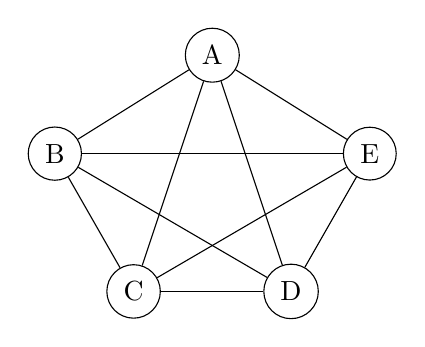
\begin{tikzpicture}
		\draw
			(0, 0) node[circle, draw] (a) {A}
			(-2, -1.25) node[circle, draw] (b) {B}
			(-1, -3) node[circle, draw] (c) {C}
			(1, -3) node[circle, draw] (d) {D}
			(2, -1.25) node[circle, draw] (e) {E};
			
		\draw (a) -- (b);	
		\draw (a) -- (d);
		\draw (a) -- (c);
		\draw (a) -- (e);
		\draw (b) -- (d);
		\draw (b) -- (e);
		\draw (b) -- (c);
		\draw (c) -- (d);
		\draw (c) -- (e);
		\draw (d) -- (e);
	\end{tikzpicture}
}
\subtable[]{
	\begin{tabular}[b]{c|ccccc}
		& \textbf{A} & \textbf{B} & \textbf{C} & \textbf{D} & \textbf{E} \\
		\hline
		\textbf{A} & 0 & 10 & 5 & 3 & 12 \\
		\textbf{B} & 10 & 0 & 6 & 8 & 10 \\
		\textbf{C} & 5 & 6 & 0 & 9 & 1 \\
		\textbf{D} & 3 & 8 & 9 & 0 & 4 \\
		\textbf{E} & 12 & 10 & 1 & 4 & 0 \\
	\end{tabular}
}
\end{figure}

\end{exercise}

Uma solução é representada pela lista ordenada de cidades. Por exemplo, um caminho que inicie na cidade \texttt{A}, siga para as cidades \texttt{B}, \texttt{C}, \texttt{D}, \texttt{E} e retorne para a cidade \texttt{A} é representada por \{A,B,C,D,E\}. Esta solução possui um custo total de 41, que é o somatório dos custos dos caminhos entre as cidades, conforme matriz de adjacências.

Mostre a execução de uma busca local simples, considerando que a vizinhança é composta pela permutação de duas posições vizinhas na solução. A seleção do vizinho utiliza a estratégia \textit{melhor melhora}. Considere como solução inicial o caminho \{A, E, B, D, C\}. Qual a solução resultante dessa busca? Trata-se de um mínimo local ou global?

Mostre a execução de uma busca local randomizada com $p = 0,2$. Cada vez que necessitar de uma decisão aleatória, considere o sorteio do próximo número da sequência abaixo. Quantas iterações a busca precisa para encontrar o ótimo global? A busca melhora se alterarmos o valor de $p$?

\begin{itemize}
	\item 0,4; 0,12; 0,08; 0,93; 0,71; 0,44; 0,1; 0,67; 0,83; 0,21; 0,09; 0;13; 0,7.
\end{itemize}

\insertspace

\begin{exercise}
Considere o problema das $N$-Rainhas com $N = 5$ (podemos chamar de problema das 5-Rainhas). O tabuleiro possui tamanho $5 \times 5$. Uma solução é representada por um vetor de inteiros $x = (r_1, r_2, r_3, r_4, r_5)$, onde $r_i$ representa a linha que a rainha $r$ ocupa na coluna $i$. A função objetivo corresponde ao número pares de rainhas que se atacam. Mostre a execução de um algoritmo genético considerando os parâmetros abaixo:
\begin{itemize}
	\item \textbf{Tamanho da população:} 5.
	\item \textbf{Função de fitness:} $1/$função objetivo.
	\item \textbf{Critério de parada:} solução encontrada (função objetivo igual a zero).
	\item \textbf{Estratégia de seleção para recombinação:} 3 melhores indivíduos.
	\item \textbf{Recombinação:} cruzamento com um ponto de corte entre $r_2$ e $r_3$.
	\item \textbf{Mutação:} troca o valor aleatoriamente de uma posição, também aleatória, da solução. O indivíduo sofre mutação com probabilidade $0.1$.
	\item \textbf{Substituição da população:} toda a população anterior é substituída pela nova população, exceto o melhor indivíduo.
\end{itemize}

\insertspace

Considere a seguinte população inicial:
\begin{itemize}
	\item $x_1 = (1, 3, 2, 4, 5)$
	\item $x_2 = (2, 3, 4, 1, 5)$
	\item $x_3 = (1, 4, 5, 2, 3)$
	\item $x_4 = (3, 4, 5, 1, 3)$
	\item $x_5 = (5, 5, 2, 3, 1)$
\end{itemize}

\insertspace

Para as decisões probabilísticas, considere a seguinte sequência de números sorteados:
\begin{itemize}
	\item 0,1; 0,4; 0,3; 0,02; 0,9; 0,05; 0,65; 0,43; 0,7; 0,1; 0,18; 0,2; 0,6; 0,85; 0,7; 0,08; 0,89.
\end{itemize}

\insertspace

Para facilitar o cáclulo do custo das soluções, pode-se utilizar o programa abaixo.

\begin{minted}{java}
public class CustoNRainhas {
	public static void main(String[] args) {
		int n = 5;
		int[] x = {5, 2, 1, 3, 4};
		int custo = 0;
		
		for(int i = 0; i < n; i++) {
			for(int j = 0; j < n; j++) {
				if(i == j) break;
				if(x[i] == x[j]) custo ++;
				
				int dif = j - i;
				if(x[i] == (x[j] + dif)) custo++;
				if(x[i] == (x[j] - dif)) custo++;
			}
		}   
		System.out.println(custo);
	}
}
\end{minted}

\end{exercise}

\begin{exercise}	
O \textbf{problema da diversidade máxima} (MDP -- \textit{Maximum Diversity Problem}) é um problema NP-Completo de otimização combinatória. Dado um conjunto de $n$ elementos, seleciona um subconjunto de $m$ elementos, tal que a diversidade entre eles seja a maior possível. Sendo $d_{ij}$ a diversidade entre os elementos $i$ e $j$ e $x_i \in \{0, 1\}$ a variável que indica se o elemento $i$ foi selecionado (valor $1$) ou não (valor $0$), podemos formalizar o problema como:
$$
\begin{aligned}
	& \text{maximiza} & & \sum_{i = 1}^{n-1} \sum_{j = i + 1}^{n} d_{ij} x_i x_j \\
	& \text{sujeito a} & & \sum_{i = 1}^{n} x_i = m, \\
	& & & x_i \in \{0, 1\}, \textbf{   } 1 \le i \le n.
\end{aligned}
$$

Uma instância do problema consiste nos valores de $n$ e $m$ e em uma matriz com os valores de diversidade $d_{ij}$ entre os elementos $i$ e $j$. A solução consiste em um vetor binário de tamanho $n$, onde a posição $i$ deste vetor indica se o elemento $i$ foi selecionado ($1$) ou não ($0$). Logo, resolver o problema significa encontrar os valores do vetor que maximizem a função objetivo dada acima. A única restrição do problema é a quantidade de elementos selecionados. Logo, a vizinhança deve ser projetada de modo a garantir que a restrição não seja violada. Mais detalhes sobre este problema podem ser consultados em \url{http://www.optsicom.es/mdp}.

Implemente uma busca local simples (subida da encosta) para o MDP. Utilize as estratégias de seleção de vizinhos Primeira Melhora -- PM e Melhor Melhora -- MM. A solução inicial deve ser gerada aleatoriamente. Faça 20 replicações de cada busca local para cada instância do problema e reporte as médias dos seguintes valores:

\begin{itemize}
	\item Tempo de execução.
	\item Número de iterações da busca.
	\item Qualidade da solução encontrada.
	\item Desvio relativo da melhor solução conhecida.
\end{itemize}

Compare os resultados das duas estratégias e comente, justificando os resultados: qual leva menos tempo para executar? Qual realiza um menor número de iterações? Qual encontra as melhores soluções? Por que as buscas não encontram soluções ótimas? Após isso, implemente alguma estratégia para fugir de mínimos locais, reportando os mesmos dados que a análise anterior e comparando com as buscas locais simples.

As \textbf{instâncias} podem ser obtidas em \url{http://www.optsicom.es/mdp}.
\begin{itemize}
	\item Utilize apenas as instâncias do conjunto \texttt{SOM-b}.
	\item $n \in \{100, 200, 300, 400, 500\}$.
	\item $m \in \{10, 20, 30, 40, 60, 80, 90, 120, 150, 160, 200\}$.
\end{itemize}

\insertspace

\textbf{Exemplo de estrutura para os resultados}

\begin{table}[h]
	\centering
	\begin{tabular}{lrrrrrr}
		\hline
		\textbf{alg} & \textbf{n} & \textbf{m} & \textbf{time (s)} & \textbf{iterations} & \textbf{value} & \textbf{dev} \\
		\hline
		PM & 100 & 10 & 0.001 & 12 & 123456.2 & 0.34 \\
		MM & 100 & 10 & 0.003 & 8 & 123123.4 & 0.22 \\
		$\vdots$ & $\vdots$ & $\vdots$ & $\vdots$ & $\vdots$ & $\vdots$ & $\vdots$ \\
		\hline
	\end{tabular}
\end{table}
\end{exercise}

\begin{exercise}
Implemente um algoritmo genético para resolver o MDP (apresentado no exercício anterior). Utilize valores de parâmetros, conforme abaixo:
\begin{itemize}
	\item \textbf{Tamanho da população:} 100.
	\item \textbf{Critério de terminação:} encontra a melhor solução conhecida ou tempo limite de 5 minutos.
	\item \textbf{Seleção para a recombinação:} seleciona 50\% da população (50 indivíduos), sendo deste os 90\% melhores (45 indivíduos) e os 10\% piores (5 indivíduos).
	\item \textbf{Recombinação:} cruzamento simples com um ponto de corte no meio da solução.
	\item \textbf{Mutação:} cada indivíduo tem 1\% de chance de sofrer mutação. A mutação substitui aleatoriamente um elemento selecionado por outro.
	\item \textbf{Substituição da população:} a nova população é composta pelos 75\% = 38 melhores indivíduos e o restante (25\% = 12 indivíduos) selecionados aleatoriamente entre os que restaram.
	\item Demais parâmetros necessários devem ser estimados empiricamente.
\end{itemize}

\insertspace

\textbf{Observação:} perceba que a recombinação de duas soluções pode gerar um descendente infactível, pois a solução deve conter exatamente $m$ elementos selecionados (posições com valor $1$). Logo, você deve desenvolver alguma estratégia para corrigir as soluções geradas que não satisfazem a restrição do problema.

Compare os resultados do algoritmo genético com os obtidos nas buscas locais do exercício anterior. Quais conclusões podem ser obtidas? Varie os parâmetros do algoritmo genético para obter um melhor desempenho. Qual o impacto de cada parâmetro na qualidade da solução encontrada?

\end{exercise}